\documentclass[a4paper]{article}

\usepackage[english]{babel}
\usepackage[utf8x]{inputenc}
\usepackage[colorinlistoftodos]{todonotes}

\title{Evolution II: Kalendr}
\author{Ellango Jothimurugesan, David Liu, Pritam Mathivanan, and Benson Tran}

\begin{document}
\maketitle

\begin{abstract}
This isn’t a research paper, but having an abstract section makes the report look polished. In any case, in this report, we are going to discuss our design choices for our calendar web application \textit{Kalendr} - spoofing Silicon Valley startups - using Django and Angular.
\end{abstract}

\section{Introduction}

In this report we will provide a retrospective on our previous design choices and their impact on completing features for this evolution, further providing insight on where such design choices made implementation feasible or a complete hassle. Moreover, we will discuss our design choices for this current evolution and elaborate on their strengths and weaknesses. In terms of front end development, we will dive into how the Angular framework provides us with a scalable architecture for a responsive and dynamic, one-page web application. In terms of back end development, we will discuss the pros and cons of how the Django REST framework may or may not have provided the most feasible outlet for developing viewsets and API endpoints. Lastly, we expand on our choices -- whether they be in the scope of frameworks, languages, database design, UI design, documentation, or teamwork -- to help us be more cognizant of better ways of tackling future evolutions.

\section{Retrospective}

This section of our report expands on how our design choices in choosing Angular.js, Django, and the Django REST Framework have set the tone and pace for implementing features in Evolution II. The learning curve for Angular.js wasn't particularly harsh, allowing front end development to focus on creating a holistic user experience. More specifically, we provided icons, buttons, animations, and responsiveness to drive the user experience. The downfall of this is that we may have been a bit too ambitious with our UI, putting heavy emphasis on aesthetics and functionality. In terms of backend development, the expectation of using the Django Rest Framework was that it would provide functionality to build a robust API; however, this framework proved problematic early on -- the dearth of online documentation didn't help either. With time we were able to code more robust, flexible viewsets.

\subsection{Front End Design Choices - Angular.js}

We initially chose Angular because of its support from Google and its lauded functionality in producing dynamic and modular .html files. Although this evolution introduced more features, we were able to scale our one-page web application relatively seamlessly. It's safe to say Angular has lived up to its hype.

\subsubsection{Seamless Functionality via Angular Directives}

We were able to introduce new features such as PUDs and groups by simply creating more Angular modules. As stated in our previous report, each Angular module can contain services, controllers, and directives. The service serves as the factory instantiating the internal API link. The controller serves as the logic that makes the application interactive to the user. Lastly, the directive is not only an unique aspect of Angular, but also has proven to be an invaluable feature used in our project. 

A directive is essentially an HTML template embedded with a bit of Angular magic. In more concrete terms, directives serve as 'front end modules', each with a specific functionality that can be embedded in the DOM. We can access directives via HTML tags. This drastically reduces the unsavvy Javascript overhead that follows with elaborate front end design and logic-heavy, one page applications.

Directives have spurred a wide variety of modules in the open-source community. This makes it possible to deploy what you want when you want. Want to have your client-sided code offload your URL routing? There's a directive for that. Want to effortlessly pass data to and from popups? There's a directive for that. We will elaborate more on the directives we've introduced in Evolution II in the latter portion of this report.

\subsubsection{Modularity and Dependency Injection}

What makes a lot of this Angular 'magic' a possibility? Modularity via dependency injection.

\begin{center}
\textit{Dependency injection is a pivotal and pervasive design pattern used in Angular applications - it provides functionality to components by providing a way for them to get a hold of their dependencies.}
\end{center}

Because Angular relies on the usage of modules, we can scale the number of modules as the number of features in our website scales. The current architecture of our front end application is only possible because of dependency injection. The highest level module, \textit{kalendr}, introduces accounts, posts, puds, etc. via dependency injection. Each of these modules introduces services, directives, and controllers via dependency injection as well.

In addition to providing a modular framework, dependency injection provides functionality to components. Directives and Angular objects are introduced through dependency injection. This is particularly pivotal if we want to maintain our one-page application. For example, we have a form for creating PUDs and a form for creating events. Each of these pop ups is associated with a controller. To propagate data to our main HTML page we need to broadcast the data from the controller of these forms to the controller associated with the main HTML page. Such communication is possible via injecting \textit{\$scope} and \textit{\$rootScope} Angular objects.

Ironically, despite Angular's reliance on modules, we've found it hard to maintain a sense of encapsulation within the project. Kalendr's main HTML page, \textit{account.html}, contains data from a variety of service factories. The main page controller \textit{account.controller.js} aggregates data from these services. The ability to inject a plethora of modules into a controller makes it hard for us not to use account controller for the majority of all functionality. Overall, we wouldn't be surprised if account controller becomes more of a bookkeeping experiment than simply a controller.

\subsection{Front End Design Choices - CSS/JS Styling Files}

Assuming the number of features increases with each upcoming evolution, it's likely that we may introduce more UI elements in our project. It's also probable that these elements will come packaged with their own stylesheets and javascript files. Although it is convenient that we can implement the functionality for these features by simply appending the path of these files into our project, this comes with drawbacks. 

Obviously, there is a performance drawback when the web page is initially loaded. The client has to download all the .js and .css files. Also, each stylesheet takes precedence over the previously loaded stylesheet, so an object can mistakenly get overridden with an unintended styling. This becomes a bookkeeping nightmare.

Before we embark on the third evolution, we plan to refactor (e.g., remove overlapping styling) and prune unnecessary stylesheets and Javascript files. Moreover, we seek to perform a UI overhaul, as a lot of our UI features aren't performing as expected.

\subsection{Back End Design Choices - Django and Django REST Framework}

The core purpose in back end development is to respond to HTTP requests generated by the client. In implementing features for this evolution, there were three major types of HTTP requests that the back end needed to handle: POST, GET, and PATCH. The back end should not only correctly serialize the data passed from the client as an object that the database can interpret, but also correctly deserialize data when requested by the client. In defining 'correct' serialization, we mean to serialize and deserialize data in such a way that it's intuitive for both front end and back end developers, in that it offloads client-sided processing, and in that it promotes less hacky solutions on all fronts of the stack.

To achieve a seamless interaction between the client and server, we need to first define the communication end between the front end and back end. In addition, we need to define how data is stored in the database and such data can be transformed in flexible ways using a variety of frameworks.

\subsubsection{Communication Interface: Django vs Django REST}

Using Django as a back end web framework, we can store data in a relational database as Django Model instances, which is managed through Django's Model APIs; any operation performed on data is done through the interface that is provided by the Django Model class. 
 
Because data is accessed as a Django class, the best way to transform the data is to package the whole class into an object; therefore, JSON became one of our natural choices. Data that is passed back and forth between front end and back end is packaged as JSON. 

Without the Django REST framework, however, we can't quite transform objects into JSON. Unfortunately, a layer of abstraction needs to be introduced to facilitate such serialization: we have to transform Django objects into native Python data structures  and then convert these structures into JSON. 

In addition to this required overhead, all communication is done through HTTP requests and responses. This means the JSON string needs to be packaged into HTTP requests and responses. 

Django Rest Framework happens to provide what we need. Django Rest Framework provides us with Response and Request classes. Request easily packages JSON. Moreover, Request can also package user information. The Request class proves to be pivotal in providing necessary data to the client.


\section{Current Design Implementation}

In this section we delve into what we believed to be three pivotal features in this current evolution: the \textit{Social Bar}, the \textit{Event Creation Request Access Rules}, and the \textit{Present-until-done Events}. Each feature is essentially a partitioned sub-project that when aggregated together fulfills the requirements for Evolution II. There were also back end and front end challenges unique to each feature. Although overcoming these challenges and implementing these features relied largely on the perceived strengths of our design and framework choices, these challenges also shed light on design flaws that may prove problematic going into future evolutions.

\subsection{Cleaning up Evolution I}

Before implementing the features for Evolution II, we pushed a lot of the processing from the client side to the server side. Initially, we had a lot of the event creation logic hacked out in Javascript, which marred the web application's performance. We also took some time to develop a more intuitive user experience. Rather than having a page of all events in chronological order, we figured it would be more intuitive to have weekly views. The user is now able to toggle to the next or previous weeks, go to a specific week, and return to the home date.


\subsection{Social Bar}

The Social Bar fulfills the groups requirement from Evolution I. Moreover, the Social Bar creates an intuitive interface by stitching event requests invitations as 'notifications' embedded in the menu. This section elaborates on the intuition behind the social system created, how its functionality is largely contingent on Angular directives and data passing, and how the development of this feature forebodes possible design malpractices in future evolutions.

\subsubsection{High-Level Description}

The Social Bar is a menu that slides out from the left of the screen. This bar contains four sections: 'Notifications', 'Followers', 'Following', 'Groups'. The Notifications section shows all event request invitations directed at the logged in user. Moreover, the user is able to respond to notifications in this accordion. The Groups section not only allows the logged in user to create groups, but also shows groups the user created and groups the user is a member of. We abided to the perennial adage, stranger danger: a member of a group has to also be the follower of the originator of said group. If a member who isn't a follower is added, that member will automatically be added as a follower. The rationale behind Followers and Following section is to show who us who has access to the logged in user's calendar and who the logged in user is following, respectively. By clicking on the users in the Following section, the logged in user is able to append or remove to her calendar the users he or she is following.

Let us remember that the Social Bar is part of the main HTML page, \textit{account.html} and its functionality is still nested in the main controller, \textit{account.controller.js}. Not surprisingly, the ability for the Social Bar to have its functionality is contingent on directives and data-binding.

\subsubsection{ngDialog Directive and Data-Binding}
ngDialog is an open source directive that makes it feasible to pass data to and from popups. When creating a popup we associate a button to that popup. The button contains ngDialog fields: \textit{ng-dialog, ng-dialog-controller, ng-dialog-data}. The field \textit{ng-dialog} connects a template HTML page for the popup, \textit{ng-dialog-controller} associates a controller to the popup, and \textit{ng-dialog-data} makes it possible to pass data from the parent scope (e.g., data associated with \textit{account.html} and \textit{account.controller.js}) to the popup. This easily introduces functionality to the popup by instantiating a controller that can inject service factories to make API calls. More importantly, ng-dialog-data is what our Social Bar is largely contingent on.

As stated before, ng-dialog-data makes data from the parent scope directly accessible from the popup's HTML template. Let us see an illustration of this by considering the life cycle of an event request notification. An event request notification is fetched via a GET request created by the Posts service factory. This factory is injected in \textit{account.controller.js} and called. The returned JSON data is displayed in \textit{account.html} via \textit{ng-model}, which introduces two-way data-binding between the controller and DOM. We can pass this binded data into our popup via ng-dialog-data. Because this popup is associated with a controller via \textit{ng-dialog-controller}, we can call an UPDATE request using the binded data to update the status of this event request notification.

\subsubsection{Too much Data and Logic in DOM and Controller?}

The type of data passing in the previous section is prevalent in our code and is also used in other features. Although Angular.js provides us with powerful tools to make our DOM dynamic and logic-filled, one could consider an overuse of these tools bad practice.

As data is passed DOM-to-DOM via HTML tags in Angular directives, this breaks the 'traditional' methodology of passing data up and down the stack via HTTP requests and allows data to flow horizontally, side-to-side. Bookkeeping becomes a problem. Where is this binded-data originally fetched from? The concept of encapsulation is essentially broken, exposing data to certain parts of the code where it shouldn't necessarily be. As with any software project, as the project scales, this free-flowing data may make team members more liable to make mistakes.

Also reading data from the DOM (originally passed in via ng-dialog-data) into a controller may provide technical difficulties. Consider the situation where one wants to call a GET request during the instantiation of the controller associated with a popup that has data binded via ng-dialog-data. This situation also requires the GET request to fetch data from ng-dialog-data.

The situation described above is analogous to a race condition seen in logic gates in Verilog design and to synchronization problems often seen in lower-level programming. Generally, race conditions are never a good idea. To fix this situation, one needs to make use of Angular object \textit{ng-init}, which is appended as an attribute to an HTML tag. 

\textit{ng-init} can set a variable in the controller to a value passed into the DOM, which in this case is passed by ng-dialog-data during the 'initialization' of the popup. Although setting a variable in the controller to ng-dialog-data should define the controller's variable during instantiation, this is rarely the case as the race condition still exists. One must \textit{ng-init} a function in the controller that takes in a parameter from ng-dialog-data. This essentially creates a lock and synchronizes the controller with the data from the DOM.

As one can tell, passing data horizontally may promote hacky, less well-developed design, and less maintainable solutions.

\subsection{Event Creation Request and Access Rules}
Event creation requests and sharing are the two most fundamental functions for this Evolution. Sharing especially is at the core of our implementation. In this section, we will discuss the implementation of our design for these features, shedding light on the structure of our back end modules.

\subsubsection{High-Level Description}
Sharing is at the core of this Evolution. To tackle this problem, first we need to define how data is stored in the database. Taking advantage of the Django framework and relational database, we use a field called \emph{"through"} for many-to-many relations. What it does is that whenever a relation is created between two objects in the database, a through field is also created to store information about this relation. With the help of through fields, we can now code information into a relation, apart from just saying those two objects are related. This through field is called \emph{AccessRule}, and the use of \emph{AccessRule}s is critical for event sharing and access control.

\subsubsection{Design and Implementation}
Let us the describe the schema of the database. Each user owns a list of events. Each user also owns a list of groups. Now, to share an event with a group or a user, we can do two things: we can either create a table for an event, and in that table, we list the usernames, group names and their \emph{visibility} (e.g., See All, Busy only, etc.), or we can  take advantage of our relational database. We can link whomever that event is shared with with that event. If later on, a user decides to change his or her name, we want that change to be reflected in all the posts that are shared with him or her. The second choice is much easier, as we do not have to go through the table every time a user updates his or her information. 

As mentioned in the \emph{High-level Description} section, we can use through fields to code information into a link that is created between two objects in the database. This is extremely useful because now we not only know that two things are related, but also can access one (type of) object through other (type of) objects that are linked to it. We can also know or specify in what way those two objects are related. 

For example, when an event is shared with a group, we can code the visibility level into that link. For example, in Figure \ref{fig:sharing1}, we have User 1 sharing an event with a group and a user, and the visibility rule is coded into the link.

\begin{figure}[h]
\centering
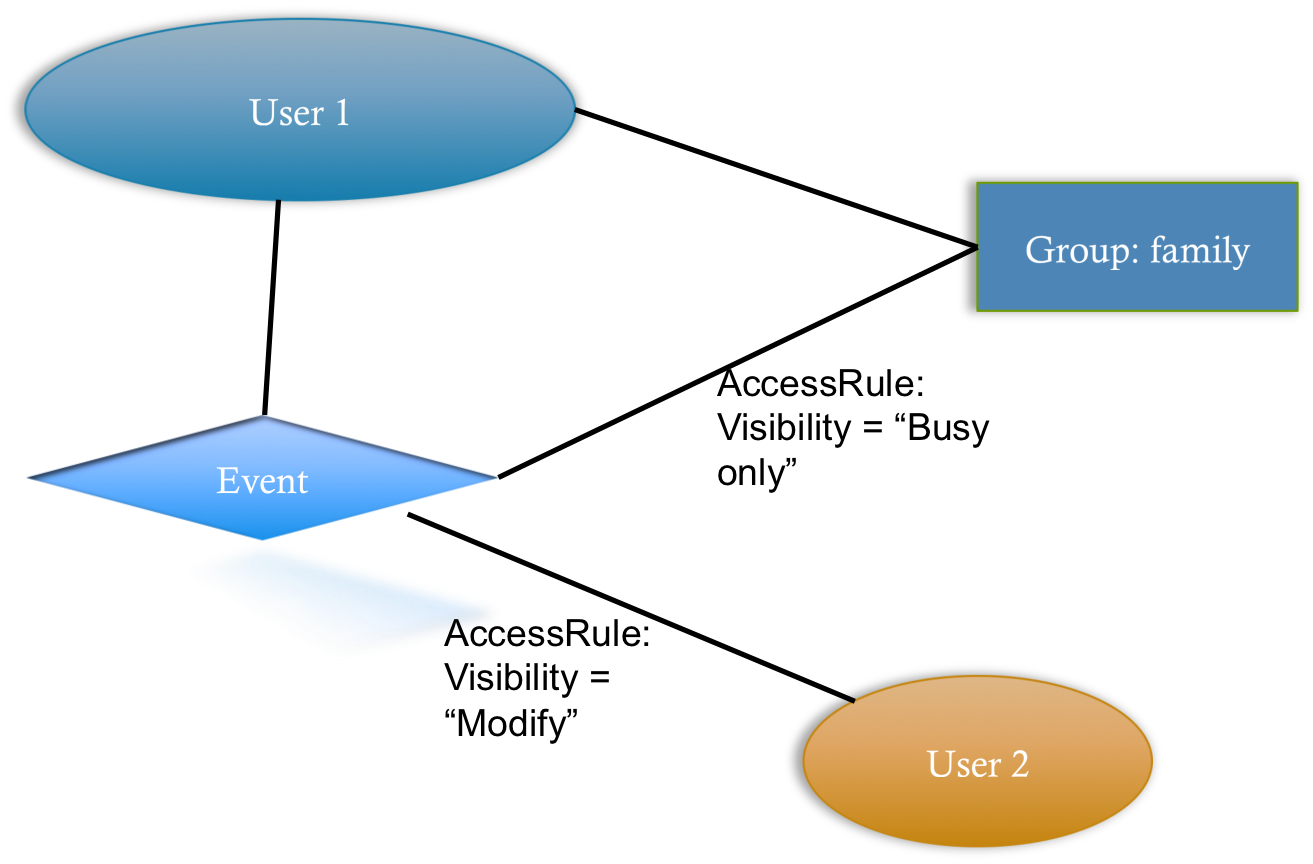
\includegraphics[width=0.5\textwidth]{sharing1.png}
\caption{\label{fig:sharing1}Basic Sharing: Visibility coded into a Relation}
\end{figure}

This use of a relational database really simplified our implementation of event creation request. An event creation event requires not only that we share events with other users, but also that the receivers respond. For example, if User 1 shares an event with User 2, then User 2 is the receiver of that sharing action. Responses can also be coded into an Access Rule. Also, to simplify the implementation of sharing, we decided that a user can only access other users through the interface of \emph{Group}. We call this type of \emph{Group}, \emph{Follower Group}. This means an event is never directly shared with a user; it is shared with a follower group that the originator owns, and the only member of that follower group is the receiver. The follower group reflects all the information about the receiver user. This way, we do not not have to worry about an event being shared with a group and then a user. Figure \ref{fig:sharing2} illustrates just this. 

\begin{figure}[h]
\centering
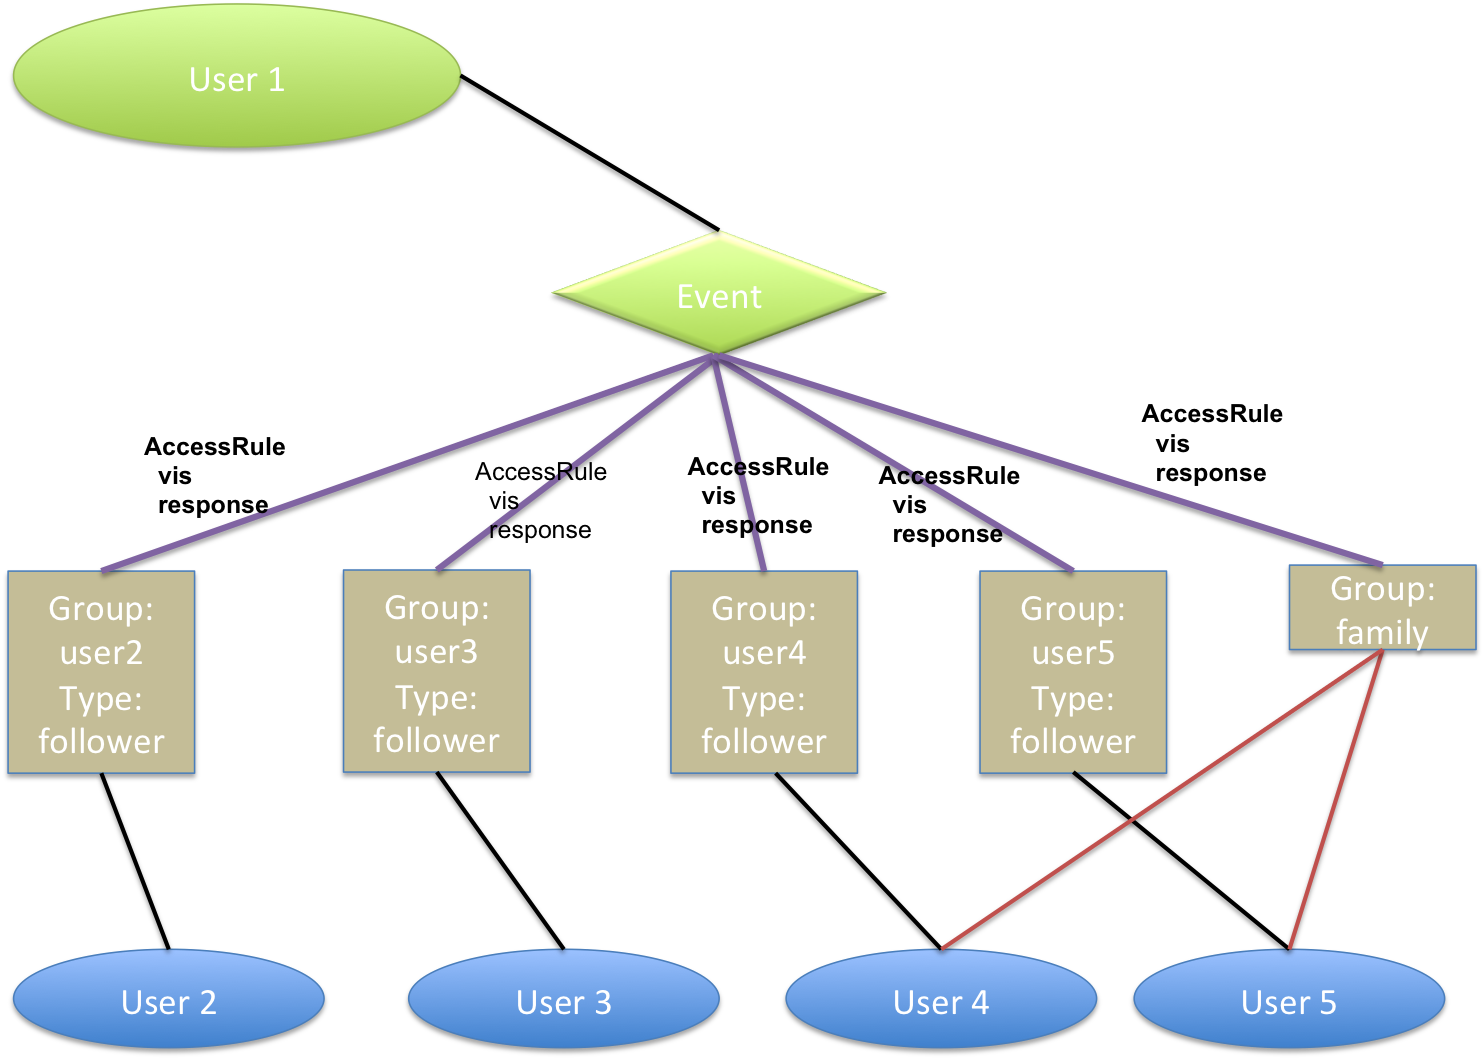
\includegraphics[width=0.4\textwidth]{sharing2.png}
\caption{\label{fig:sharing2}AccessRule, follower groups and sharing}
\end{figure}

Another benefit of this idea is that when an event is shared with a [\emph{non-follower}] group, every member of that group can get a chance to reply to that request because the event is really shared with a list follower groups. The aggregation of the members of these follower groups creates the members of the overarching non-follower group. 

This design is opaque to other parts of the system. For example, when the front-end gives a request to share an event with a user, it still issues the same command. To the outside world, it is as if the event is shared with an individual user directly.

\subsubsection{Model, Serializer and ViewSet}
Access rules, follower groups and sharing is implemented as a Django Model. It is worth noting again the framework that Django lays out (See Figure \ref{fig:basicstructure}). Models define the database schema. In other words, models not only define tables in the database, but also define the type of columns and how many columns there are in each table. \emph{Serializer} is responsible for conversion between JSON data and model instances. ViewSets provide API endpoints for the front-end to call through HTTP requests. Viewsets handle HTTP requests and respond with HTTP responses. 

\begin{figure}[h]
\centering
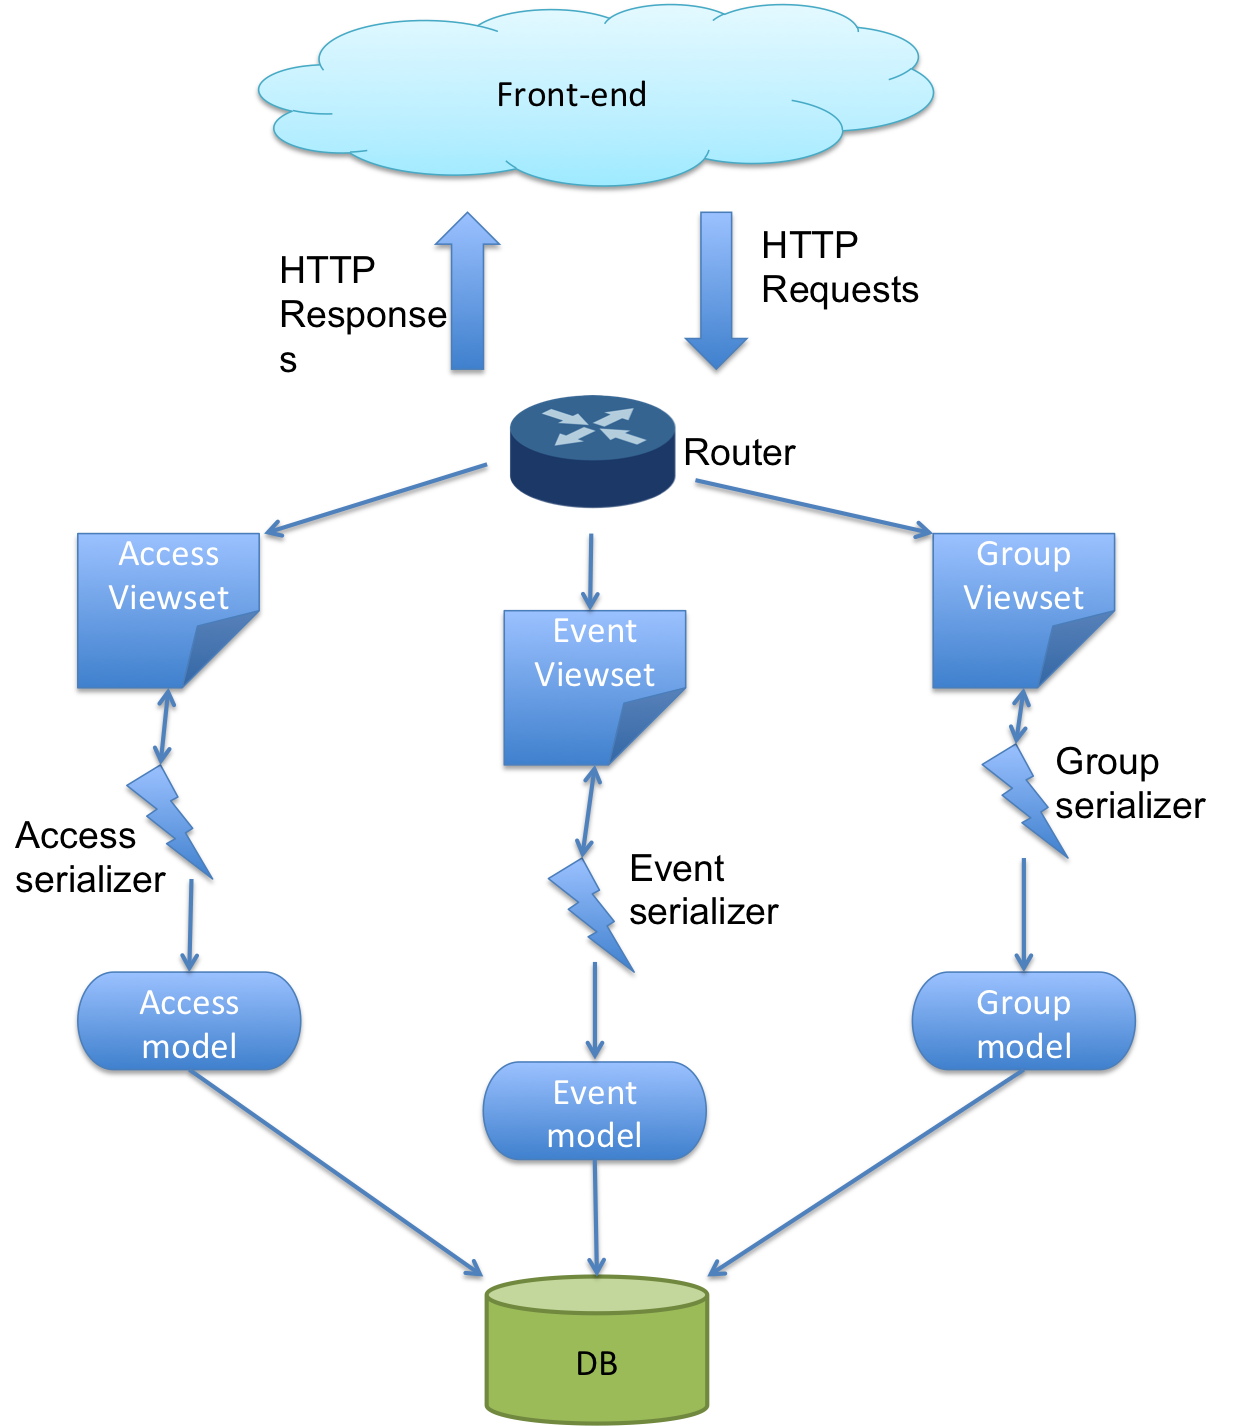
\includegraphics[width=0.5\textwidth]{basic_structure.png}
\caption{\label{fig:basicstructure}Basic Architecture of Kalendr}
\end{figure}

Therefore, with the database schema laid out, most of the logic is in implementing Viewsets. The goal of our back-end implementation is to minimize the logic in the front-end. Ideally, the front-end can almost mindlessly call an API that the back-end provides and achieve whatever it wants to do. For example, if the front-end wants to display a list of users who have not responded to an event creation request, it should be able to call an API call and acquire said list of users.

\subsection{Present-until-done Events}

\subsubsection{High-Level Description}

Present-until-done events (PUDs) are visualized on a screen, from here on referred to as the "pudscreen", that overlays the main calendar interface. There are three columns, which will be marked for user-friendliness: This Week, This Month, and By Priority. The PUDs are sorted and added dynamically into the "This Week" and "This Month" columns, whereas all PUDs are added to the "By Priority" column. The "By Priority" columns displays PUDs in descending order of priority, and for PUDs with the same priority level, the PUD with the oldest creation time is displayed first.

A user can create a PUD by clicking the button with the pen image. The button click will produce a form, on which the user can assign the various attributes of a PUD. The structure of the displayed PUD is rather simple, listing the content, duration, repeat interval, priority and completion check box. One can access the pudscreen by clicking the button with the check image.

As required by the evolution, a user has the capability to create calendar events hosting work time for the highest priority PUD that is yet to be completed. Completing a PUD, via clicking the check box, will remove the PUD from the pudscreen and update any posts that were hosting the just-completed PUD.

All of the PUD .html markup is located within account.html and logic concerning PUD creation and completion is handled by \emph{account.controller.js}. Data-binding and Django querysets were the key players in making PUDs a reality.

\subsubsection{Data-binding and Django Querysets}

The AngularJS directives and controllers for PUDs were largely similar to the directives and controllers for creating calendar events. The major changes were in the render functions used to display the PUDs. For PUDs, the major difficulty was in associating a calendar event with a specific PUD. There is no simple way to pass PUD data to a calendar event, and thus, we had to configure database URLs to make changes directly on the event model. AngularJS is often praised and criticized for its ability to pass data around on the front-end; however, the value of the passed data is not always clear, for we witnessed many "undefined" value errors. As such, the most viable and reliable option was to query for the appropriate PUD in an event's backend logic classes, known as ViewSets. Using an event ViewSet, it is rather easy to filter for and obtain the desired PUD, and in reverse, using a PUD ViewSet, it becomes easy to update all associated events. Abstractly, this can be thought of as a pseudo-data-binding/passing. The downside of ViewSets is that they cannot pass data amongst themselves, since ViewSets always return serialized data in a http response. Therefore there is a lot of back and forth http.post and http.get requests occurring while trying to mold the relationship between PUDs and events.

Interestingly enough, calling multiple http.post and http.get requests in succession is not necessarily bad practice, and is much more sustainable than horizontal data passing on the front end. The weakness of numerous requests is obviously the load on the server, which will certainly slow down a single page application that is listening for numerous signals, most of which further call http.post and http.get requests for updating and displaying data.

In the future, we hope to implement a socket system such that we can consistently listen to changes in the database. By watching the database change in real time, we reduce the size of the data that must be retrieved or needs to be saved. Essentially, the application can update state with incremental data without having to reload the whole DOM to assess the data in a GET or POST request.


\section{Individual Contributions}
\subsection{Ellango}
In this evolution, Ellango primarily worked with his team on implementing the back end of groups and event creation requests. He designed an experiment to test his back end code by writing scripts that execute the API calls to create groups and share events, with assert statements to verify the expected state changes were occurring, or to reveal problems if they existed. From these scripts, he was able to determine what bugs were present. Unfortunately these scripts became out of date as the project evolved, and he abandoned them, rather than maintaining them to use as a test for whether changes in the code preserve the functionality. He hopes to have living test scripts for the future.

A system component he designed was the module responsible for sending email reminders for events and PUDs. The task of sending emails immediately after a user creates an event is trivial within the Django framework. The challenge was in managing queues of emails to send at user-specified times and in doing so until the event is complete. After initial struggles with workaround hacks to do something Django was not designed for, he did some research found that he was able to offload essentially all of the heavy lifting to a third-party service, Mandrill. In this way, he was able to complete the email feature much faster and spend time on other required features for the evolution.

Ellango worked with his team by meeting with them regularly to share updates about their progress and obstacles. This was far more efficient than trying to resolve issues remotely.

\subsection{David}
David was responsible for most of the functionality in the back end. For this Evolution, he mostly worked on implementing, testing and improving API endpoints for the front end to call. The list of API endpoints he implemented includes creating, updating \emph{AccessRule}, fetching a list of users according to their responses to an event creation request, updating event information, fetching a list of events to which a user needs to respond, fetching other users' events according to their visibility rules, etc.

To implement those functionalities, David had to do extensive testing on the system in order to make sure all interfaces are well-defined and implemented and all components are connected correctly. For example, when implementing the functionality of getting a list of users according to their responses to an event creation request, David examined the front-end code where the HTTP request is made to make sure that the correct API is requested. He then analyzed the traces generated by the code to make sure all data are serialized correctly. He also examined the error generated by the web server to check potential server configuration problem. And it is in the web server error messages, David found that there was a variable name mismatch that was causing the problem. 

Ellango and David designed the back-end database schema together. One design decision they made in terms of sharing was the usage of follower groups (example described in \textbf{Section 3.3}). Because each model defined must have a table in the database, using inheritance is hardly an clean option. So in order to avoid making repeated code for handling sharing with groups and users, they made the decision that users can only be accessed through the interface of groups. Thus the idea of follower groups were created. This way, events are only shared with groups. This decision only concerns with the database schema, to work around the restriction of not being able to use inheritance easily. For other parts of the system, this decision is hidden. When an event is shared with a user, the event does not know that it is linked with a different type of group.

David worked closely with front-end team, asking what type of API endpoints would best serve their needs and explaining how to use those API endpoints. He did pair programming with teammates to resolve bugs and issues.
\subsection{Pritam}

Pritam was the mastermind behind PUDs. He received scaffolding help with the PUD controller structure from Benson. Pritam wrote numerous url routers to access new logic functions in the event and PUD models to manipulate the association between each of the two objects. He designed the backend logic functions so that they would assist in dynamically updating specific DOM elements. His main testing tool was the Python console, in which he wrote several testing scripts to assert the values of PUDs and events hosting PUDs. He also designed the visual layout structure for PUDs. 

He also analyzed the traceback for all http GET and POST requests to make sure the server wasn't being overloaded. He did note that there was not a clear way to force pairs of GET and POST requests to complete in sequence, indicating that data is being passed around at inappropriate times. There are however, no visual changes to be noted because of these mis-ordered http requests.

In dealing with realistic constraints, Pritam put PUD repetition and PUD emails on the backburner, since it would be better to combine repeat and email code for events and PUDs and then refactor to produce robust, bug-free logic.

Pritam also created the seven column display with banners representing empty days. Working alongside Benson, the decision was made to make the application more intuitive after attempting to be too innovative with the chronological calendar in Evolution I.

Pritam communicated with his team through Facebook and class, and was diligent in organizing meeting times and booking rooms to work in. He performed a project rebuild, hosting a new 'kalendr' repository on github.com as soon as Evolution II was released. This new repository was necessary because there were many corrupt files in the previous repository which had not been pruned correctly by .gitignore.
\subsection{Benson}

Benson's responsibilities were largely in the scope of front end development and high-level project design. He initially cleaned up, refactored, and improved the performance and functionality of Evolution I's features. Rather than having a chronological view of all events on the page, he implemented a weekly view with features to scroll to the previous and next weeks, to change dates, and to return to today's date. Because fewer events were shown, there were clear improvements in performance. Also a lot of the front end processing of repeating events was sent to the back end, further improving performance.

He also had the responsibility of implementing the Social Bar. The idea of the Social Bar was to provide an intuitive interface for anything social, whether it be creating groups, viewing group information, or replying to event notifications. One cool feature of the Social Bar was the autocomplete feature in searching for users. Using an open-source Angular directive, the autocomplete feature queries the back end for possible users.

To provide a seamless one-paged web application, Benson used lots of popups, AJAXing calls, and data passing. Asynchronous GET requests lead to inconsistency with data-binding to the DOM, which prevented dynamic rendering in some areas (e.g., responding to notifications doesn't remove the notification unless the page is refreshed). Sockets may be used in future evolutions to rectify such issue.

Lastly, pair-programming with David was pivotal in getting the Social Bar up-and-ready in time. Not to beat a dead horse, but pair-programming reduced the ambiguity in what was required by both parties. One can make the argument that laying out a solid API from the get-go would provide the same benefit; however, Benson begs to differ. Being novices at these frameworks, the team felt that it would be better to tackle problems together. By doing so, they would better understand the limitations of particular viewsets in the back-end and of certain directives in the front end. A robust API is required to produce fully-fledged functionality in features. A robust API is only built through ongoing communication as opposed to initially laying out a doctrine.

\end{document}